%!TEX root = ../main.tex

\section{Modeling approach}

Engineering correlations, reduced-order models, and CFD modeling techniques were used to investigate the effects of recycled gas on the operation of a fluidized-bed biomass pyrolysis reactor. The following sections discuss approaches implemented in this work for calculating gas properties and the associated effects on fluidization conditions and pyrolysis yields.

\subsection{Gas properties}

Density of the gas is calculated from the ideal gas law as shown in Equation \ref{eq:density} where $\rho_{gas}$ is density (kg/m$^3$), $P$ is pressure (Pa), $MW$ is molecular weight (g/mol), $R$ is the gas constant [(m$^3$ Pa) / (K mol)], and $T$ is temperature (K).

\begin{equation}\label{eq:density}
    \rho_{gas} = \frac{P\,MW}{R\,T}
\end{equation}

Gas viscosity ($\mu_{gas}$ as \textmugreek P) is determined from Equation \ref{eq:viscosity}, thermal conductivity ($k_{gas}$ as W/m\,K) is estimated from Equation \ref{eq:thermlcond}, and heat capacity (C$_{p\,gas}$ as J/mol\,K) is calculated from Equation \ref{eq:heatcap}. Temperature of the gas in Kelvin is represented by $T$ while the regression coefficients $A$, $B$, $C$, $D$, $E$, $F$, and $G$ for each gas are obtained from Yaws' Handbook \cite{Yaws2014}.

\begin{equation}\label{eq:viscosity}
    \mu_{gas} = A + B\,T + C\,T^2 + D\,T^3
\end{equation}

\begin{equation}\label{eq:thermlcond}
    k_{gas} = A + B\,T + C\,T^2 + D\,T^3
\end{equation}

\begin{equation}\label{eq:heatcap}
    C_{p\,gas} = A + B\,T + C\,T^2 + D\,T^3 + E\,T^4 + F\,T^5 + G\,T^6
\end{equation}

Several methods are available to calculate the viscosity of a gas mixture. Equation \ref{eq:graham} calculates the mixture viscosity from the sum of the mole fraction and viscosity product of each gas component in the mixture \cite{Graham-1846} while Equation \ref{eq:herning} accounts for the molecular weight of each gas component \cite{Herning-1936}.

\begin{equation}\label{eq:graham}
    \mu_{mix} = \sum(x_i \cdot \mu_i)
\end{equation}

\begin{equation}\label{eq:herning}
    \mu_{mix} = \frac{\sum(\mu_i \cdot x_i \cdot \sqrt{MW_i})}{\sum(x_i \cdot \sqrt{MW_i})}
\end{equation}

\subsection{Fluidization correlations}

For a bed of particles, the minimum fluidization velocity $U_{mf}$ is the gas velocity at which the drag force of the upward moving gas equals the weight of the particles. Kunii and Levenspiel \cite{Levenspiel-1991} provide the following equation for calculating minimum fluidization velocity

\begin{equation}
    U_{mf} = \frac{Re_{p,mf} \mu}{d_p \rho_g}
\end{equation}

\noindent where $\mu$ is gas viscosity (kg/m\,s), $d_p$ is particle diameter (m), $\rho_g$ is gas density (kg/m$^3$), and $Re_{p,mf}$ is the particle Reynolds number (-) at minimum fluidization conditions. The Reynolds number is calculated from the Archimedes number ($Ar$) and two dimensionless constants ($a, b$) which represent experimental coefficients. Different $U_{mf}$ correlations were evalutaed based on experimental data from Wen and Yu where $(a, b) = (33.7, 0.0408)$, from Richardson where $(a, b) = (25.7, 0.0365)$, and from Grace where $(a, b) = (27.2, 0.0408)$ \cite{Levenspiel-1991}.

\begin{align}
    Re_{p,mf} &= \left( a^2 + b Ar \right)^{1/2} - a \\
    Ar &= \frac{d_p^3 \rho_g (\rho_s - \rho_g) g}{\mu^2}
\end{align}

According to Kunii and Levenspiel \cite{Levenspiel-1991}, the constants ($a, b$) can be derived from the Ergun pressure drop equation based on the constants $K_1$ and $K_2$ where $\epsilon_{mf}$ is the bed void fraction (-) at minimum fluidization and $\phi$ is sphericity (-) of the bed particles. For this paper, $U_{mf}$ is estimated based on the Ergun, Grace, Richardson, and Wen and Yu correlations.

\begin{equation}
    a = \frac{K_2}{2 K_1} \qquad
    b = \frac{1}{K_1}
\end{equation}

\begin{equation}
    K_1 = \frac{1.75}{\epsilon_{mf}^3 \phi} \qquad
    K_2 = \frac{150(1-\epsilon_{mf})}{\epsilon_{mf}^3 \phi^2}
\end{equation}

\subsection{Pyrolysis kinetics}

A pyrolysis kinetics scheme based on the work of Di Blasi was implemented to predict the conversion of biomass into gas, tar, and char products \cite{Blasi-1993,Blasi-2001}. Figure \ref{fig:blasi} gives an overview of the scheme and its reaction mechanisms. Reactions 1--3 represent the primary conversion of biomass while reactions 4--5 are secondary reactions that reduce tar yield at long residence times.

\begin{figure}[H]
    \centering
    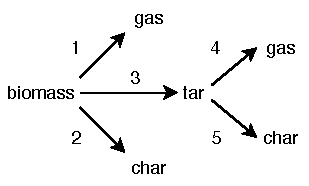
\includegraphics[width=0.4\textwidth]{blasi.pdf}
    \caption{Diagram of the Di Blasi pyrolysis kinetics scheme for conversion of biomass to gas, tar, and char products.}
    \label{fig:blasi}
\end{figure}

The pyrolysis reactions were modeled as first-order Arrhenius type equations where the reaction rate is given as

\begin{equation}
    r_i = C_i\,A_i\,e^{-E_i / R\,T}
\end{equation}

\noindent where $r_i$ is the rate of reaction $i$ such that $C_i$ is a mass based concentration, $A_i$ is the pre-factor (1/s), $E_i$ is the activation energy (kJ/mol), $R$ is the gas constant, and $T$ is the reaction temperature (K). Kinetic parameters for each reaction are listed in Table \ref{tab:kinetic-params}.

\begin{table}[H]
    \centering
    \caption{Kinetic parameters for the Di Blasi biomass pyrolysis scheme.}
    \begin{tabular}{cllc}
        \toprule
        Reaction    & A (1/s)               & E (kJ/mol)    & Reference     \\
        \midrule
        1           & $4.38 \times 10^9$    & 152.7         & \cite{Blasi-2001} \\
        2           & $3.27 \times 10^6$    & 111.7         & \cite{Blasi-2001} \\
        3           & $1.08 \times 10^{10}$ & 148.0         & \cite{Blasi-2001} \\
        4           & $4.28 \times 10^6$    & 108.0         & \cite{Blasi-1993} \\
        5           & $1.00 \times 10^6$    & 108.0         & \cite{Blasi-1993} \\
        \bottomrule
    \end{tabular}
    \label{tab:kinetic-params}
\end{table}

\subsection{Parameters}

Parameters for the reduced-order model and CFD simulations are provided in Tables \ref{tab:params-particle} and \ref{tab:params-reactor}. Biomass particle characteristics and properties are representative of loblolly pine. Bed particle characteristics are for typical sand material. Operating conditions and reactor dimensions are based on the previously discussed NREL 2FBR fluidized bed pyrolysis unit.

\begin{table}[H]
    \centering
    \caption{Particle parameters for the biomass and bed material (sand). Diameters represent the Sauter-mean diameter.}
    \label{tab:params-particle}
    \begin{tabular}{lrll}
        \toprule
        Parameter & Value & Units & Description \\
        \midrule
        d$_\textrm{p\,bed}$          & 235    & \textmugreek m  & bed particle diameter        \\
        \straightphi$_\textrm{bed}$  & 0.86   & --              & bed particle sphericity      \\
        \textrho$_\textrm{bed}$      & 2,500  & kg/m$^3$        & bed particle density         \\
        d$_\textrm{p\,bio}$          & 135    & \textmugreek m  & biomass particle diameter    \\
        \straightphi$_\textrm{bio}$  & 0.0    & --              & biomass particle sphericity  \\
        \textrho$_\textrm{bio}$      & 540    & kg/m$^3$        & biomass particle density     \\
        \bottomrule
    \end{tabular}
\end{table}

\begin{table}[H]
    \centering
    \caption{Reactor parameters for the bubbling fluidized bed pyrolysis reactor.}
    \label{tab:params-reactor}
    \begin{tabular}{lrll}
        \toprule
        Parameter & Value & Units & Description \\
        \midrule
        d$_\textrm{inner}$    & 5.25     & cm   & inner reactor diameter  \\
        H$_\textrm{reactor}$  & 43.18    & cm   & reactor height          \\
        H$_\textrm{static}$   & 10.16    & cm   & static bed height       \\
        P$_\textrm{gas}$      & 101.325  & kPa  & gas pressure            \\
        T$_\textrm{gas}$      & 773.15   & K    & gas temperature         \\
        Q$_\textrm{gas}$      & 14       & SLM  & inlet gas flowrate      \\
        \bottomrule
    \end{tabular}
\end{table}

\subsection{Simulation cases}

Table \ref{tab:cases} represents the CFD simulations conducted for this paper. Each row is for a different simulation case which is performed for a particular gas composition.

\begin{table}[H]
    \centering
    \caption{Simulation cases for different gas mixtures where columns denote gas percentage.}
    \begin{tabular}{crrrrrr}
        \hline
        Case    & N$_2$ & H$_2$     & H$_2$O    & CO    & CO$_2$    & CH$_4$    \\
        \hline
        1       & 100   & 0         & 0         & 0     & 0         & 0         \\
        2       & 0     & 100       & 0         & 0     & 0         & 0         \\
        3       & 0     & 0         & 100       & 0     & 0         & 0         \\
        4       & 0     & 0         & 0         & 100   & 0         & 0         \\
        5       & 0     & 0         & 0         & 0     & 100       & 0         \\
        6       & 0     & 0         & 0         & 0     & 0         & 100       \\
        7       & 20    & 20        & 0         & 20    & 20        & 20        \\
        8       & 50    & 0         & 0         & 0     & 50        & 0         \\
        9       & 50    & 0         & 0         & 50    & 0         & 0         \\
        10      & 0     & 0         & 50        & 50    & 0         & 0         \\
        11      & 100   & 0         & 0         & 0     & 0         & 0         \\
        12      & 80    & 20        & 0         & 0     & 0         & 0         \\
        13      & 60    & 40        & 0         & 0     & 0         & 0         \\
        14      & 50    & 50        & 0         & 0     & 0         & 0         \\
        15      & 40    & 60        & 0         & 0     & 0         & 0         \\
        16      & 30    & 70        & 0         & 0     & 0         & 0         \\
        17      & 20    & 80        & 0         & 0     & 0         & 0         \\
        18      & 15    & 85        & 0         & 0     & 0         & 0         \\
        19      & 10    & 90        & 0         & 0     & 0         & 0         \\
        20      & 5     & 95        & 0         & 0     & 0         & 0         \\
        21      & 0     & 100       & 0         & 0     & 0         & 0         \\
        \hline
    \end{tabular}
    \label{tab:cases}
\end{table}
